% Diese Zeile Bitte -nicht- aendern.
\documentclass[course=erap]{aspdoc}
\usepackage{amssymb}
\usepackage{amsmath}
\usepackage{xcolor}
%%%%%%%%%%%%%%%%%%%%%%%%%%%%%%%%%
\newcommand{\theGroup}{128} % Beispiel: 42
\newcommand{\theNumber}{A220} % Beispiel: A123
\author{Ashkan Hassani \and Aosimanjiang Aihaiti \and Konrad Schlüter}
\date{Wintersemester 2023/24} % Beispiel: Wintersemester 2019/20
%%%%%%%%%%%%%%%%%%%%%%%%%%%%%%%%%

% Diese Zeile Bitte -nicht- aendern.
\title{Gruppe \theGroup{} -- Bildentrauschung \theNumber}

\begin{document}
\maketitle

\section{Einleitung}
%\subsection{Überblick}
Bildentrauschung bezeichnet den Prozess der Reduzierung oder Beseitigung von Rauschen in digitalen Bildern. 
Rauschen kann durch verschiedene Faktoren wie schlechte Lichtverhältnisse, Sensorfehler oder bei der Bildübertragung entstehen. 
Die Herausforderung besteht darin, Algorithmen zu entwickeln, die ohne Verlust von wichtigen Bildinformationen Rauschen reduzieren. Nach der Entwicklung einer funktionsfähigen Implementierung wird diese auf Laufzeit optimiert und die resultierenden Implementierungen verglichen.


\section{Lösungsansatz}

\subsection{Netpbm}
Netpbm ist ein Open-Source-Paket, bestehend aus Grafikprogrammen und einer Programmierbibliothek. Das Paket enthält über 330 einzelne Programme, von denen die meisten \texttt{pbm}, \texttt{pgm}, \texttt{ppm}, \texttt{pam} oder \texttt{pnm} im Namen tragen, und mit diesen Formaten arbeiten.
Jedes Netpbm File hat einen Header, in dem die Eigenschaften des Files beschrieben sind\cite{netpbm}. Es enthält:
\begin{itemize}
    \item \textbf{Magic Number} : Diese Nummer besteht aus zwei Zeichen, nämlich dem Buchstaben \texttt{p} und einer Zahl von 1 bis 6, die den Dateityp identifiziert. 
    \item \textbf{Width} und \textbf{Height} : Diese zwei Zahlen bestimmen Breite und Höhe des Bildes. 
    \item \textbf{MaxValue} : Diese Nummer ist codiert ASCII dezimal den maximalen Farb- bzw. Helligkeitswert jedes Pixels.
\end{itemize} 

\subsection{Allgemeine Funktionsweise}

Der Bildentrauschungsalgorithmus wird in drei Schritten realisiert. 
\begin{enumerate}
    \item\textbf{Graustufenkonvertierung} \newline
    %definition ein 24bpp PPM Image und PGM Image 
    Das geeignete Bildformat für Ausgabefile bei Bildentrauschung ist PGM (Portable GrayMap), da es  für die Graustufenbilder lediglich 8 oder 16Bits pro Pixel verwendet und dadurch die Verarbeitung der Bilddaten vereinfacht, wobei es sich leicht in andere Formate  konvertieren lässt und kompatibler mit meisten Bildbearbeitungsprogrammen und auf der anderen Seite speicher- und recheneffizient ist. 
    Im PPM (Portable PixMap) Bildformat wird jedes Farbpixel an der Position $(x,y)$ mit 24 Bits definiert, in dem die 3 Farbkanälen Rot(R), Grün(G) und Blau(B) jeweils unterschiedliche 8-Bit-Ganzzahlenwerte haben.
    \newline
    Die Konvertierung eines Farbpixels in Graustufen wird mittels Division erledigt. 
    %\item \textbf{{Funktionsweise}} 
    \newline
    Das Bildbearbeitungsprogramm GIMP verfügt über drei Algorithmen. \newline
    Die \textbf{Helligkeitsmethode}, welche den Durchschnitt der auffälligsten und am wenigsten auffälligen Farben bildet. %: $$  D = \frac{max(R, G, B) + min(R, G, B)}{2}$$ 
    Die \textbf{Durchschnittsmethode}, bei der die Werte einfach gemittelt werden %: $$D = \frac{R + G + B}{3}$$
    und die \textbf{Luminanzmethode}, welche eine anspruchsvollere Version der Durchschnittsmethode ist.
    Mittel dieses Algorithmus wird einen gewichteten Durchschnitt von 3 Farbkanälen berechnet und eingesetzt, wobei die folgende Gleichung benutzt wird:
        $$ D = \frac{a\cdot R + b\cdot G + c\cdot B}{a + b + c}   $$
     in der die Variablen a, b und c frei wählbare Zahlen sind.\newline
     Das entsprechende Pixel in Graustufen für jede Position ist dann gegeben durch $$ Q_{(x, y)} = D $$
\begin{itemize}
   \item\textbf{a, b, c Werte} \newline 
    Die drei Koeffizienten a, b und c repräsentieren die Helligkeitswahrnehmung von Menschen gegenüber Licht. Die menschliche Wahrnehmung ist am empfindlichsten für Grün und man sieht diese Farbe normalerweise besser als die anderen. Die ITU (International Telecommunication Union) empfiehlt die folgenden Werte\cite{grayscaleCoeff}:
    $$ a = 0.2126 , \: b = 0.7152 , \: c = 0.0722 $$ 
    Bei diesen Zahlen ist zu beobachten, dass sie in Summe Eins ergeben, man spart sich also die Division und damit Laufzeit.
    \end{itemize}
\item \textbf{Faltung} \newline
    In der Bildverarbeitung wird die diskrete Faltung verwendet, um Filteroperationen auf Bildern durchzuführen. Es handelt sich meist um eine quadratische Matrix und eine lineare Operation. Die diskrete zweidimensionale Faltung für Bildbearbeitung ist definiert als 
    \[
    I^*(x,y) = \sum_{i=1}^{n}\sum_{j=1}^{n} I(x-i+a,j-y+a)k(i,j)
    \]
    wobei \texttt{i} und \texttt{j} in unserem Fall von \texttt{-1} bis \texttt{1} laufen und ein Zugriff außerhalb des Definitionsbereichs der Funktionen implizit den Wert 0 annimmt. \newline
    Das Graustufenbild wird zwei Faltungen unterzogen, wodurch Kantendetektion $Q^L$ und Weichzeichnung $Q^W$ realisiert werden.
\begin{itemize}
   \item \textbf{Weichzeichnung} \newline
    Die Weichzeichnung eines Bildes ist eine Bildverarbeitungstechnik, die dazu verwendet wird, Bildrauschen zu reduzieren. Der Mechanismus dahinter liegt darin, dass die Pixelwerte in einem lokalen Bereich gemittelt werden. Dies führt dazu, dass kleinere zufällige Schwankungen in den Pixelwerten eliminiert werden. Besonders effektiv ist der Gauß'sche Weichzeichnungsfilter (der Dimension 3) \texttt{$M^W$}, der eine gewichtete Mittelwertbildung verwendet. Dieser wird auf das Graustufenbild $Q$ wie gefolgt angewendet:
    \[
        Q^W = \frac{1}{16}\cdot M^W\ast Q \text{ mit } M^W = \begin{pmatrix}
            1 & 2 & 1 \\ 2 & 4 & 2 \\ 1 & 2 & 1
        \end{pmatrix}
    \]
    Jedoch geht diese Rauschreduzierung nicht ohne Konsequenzen vonstatten. Die Weichzeichnung verringert auch die Bildauflösung, da die scharfen Übergänge zwischen unterschiedlichen Strukturen im Bild abgeschwächt werden. Das heißt, feine Details wie Kanten werden unschärfer.

    \item\textbf{Kantendetektion} \newline
    % Laplace-Filter und sein Zweck
    Der Laplace Filter betont Unterschiede in der Intensität zwischen benachbarten Pixeln und eignet sich gut für die Kantendetektion. Der diskrete 2D-Laplace-Filter wird $M^L$ auf das Graustufenbild $Q$ folgenderweise angewendet:
    \[
        Q^L \approx M^L\ast Q \text{ mit } M^L= \begin{pmatrix}
        0&1&0 \\ 1&-4&1 \\ 0&1&0
        \end{pmatrix}
    \]
\end{itemize}
    \item \textbf{Zusammensetzung} \newline 
    Das entrauschte Bild entsteht, indem man das Graustufenbild $Q$, das Ergebnis von Weichzeichnung $Q^W$ und das Ergebnis der Kantendetektion $Q^L$ wie folgt zusammenführt:
    \[
    Q'_{(x,y)} = \frac{|Q^L_{(x,y)}|}{1020}\cdot Q_{(x,y)}+(1-\frac{|Q^L_{(x,y)}|}{1020})\cdot Q^W_{(x,y)}
    \]  
    Die Vorteile dieser Kombination liegen in der gezielten Berücksichtigung von Kanten. Durch die Gewichtung mit $|Q^L_{x,y}|$ wird der Einfluss des Ursprungsbildes verstärkt, wenn Kanten vorhanden sind, während in glatten Bereichen die Weichzeichnung stärker berücksichtigt wird. Dies führt zu einer ausgewogenen Rauschreduzierung, wobei wichtige Details, insbesondere Kanten, besser erhalten bleiben.
\end{enumerate}
\subsection{Implementierungen}
In \texttt{image} sind Funktionen für Lesen und Schreiben eines PPM bzw. PGM Files definiert. \texttt{read\_image} liest die Inhalte eines PPM File und \texttt{write\_image} schreibt ein PGM File als Output, wobei die beiden Funktionen dem Netpbm Standard folgen. \newline Die gelesenen Inhalte werden im nächsten Schritt mittels der Methode \texttt{denoise} abgearbeitet. \texttt{Denoise} führt den Bildbearbeitungsprozess mithilfe von 3 Hauptfunktionen durch, indem nacheinander $\textbf{grayscale}$, $\textbf{convolution}$ (Faltungen), und $\textbf{combine}$ aufgerufen werden. \newline Am Ende wird mittels \texttt{write\_image} das Output-File im \texttt{pgm} Format gespeichert.

\subsubsection{Akkurate Implementierung}
% Änderung an Laplace um die elemente als 8 Bit integer zwischenzuspeichern
% Und Auswirkung auf combine 
Die akkurate Implementierung repräsentiert eine naive Implementierung der beschriebenen Methode zur Entrauschung der Bilder ohne Optimierungen. In dieser Implementierung basieren alle Arithmetik Operationen auf Fließkommazahlen-Arithmetik und liefert deshalb ein Endergebnis, bei dem alle Pixelwerte möglichst akkurat sind. \newline 
Bei \texttt{grayscale} wird durch die Pixel iteriert und die Luminanzmethode zur Berechnung jedes Graustufenpixels verwendet.\newline Im Anschluss finden die Faltungen statt. Zuerst wird der Laplace Filter auf das Graustufenbild angewendet: Es werden alle Pixel durchlaufen, und jeweils die Pixel einer 3x3-Nachbarschaft mit den korrespondierenden Werten der Filtermatrix multipliziert. Anschließend werden diese 9 Werte zusammenaddiert und als Ergebnis des Pixels gespeichert. Eine Eigenschaft vom Laplace-Filter ist, dass die Pixelwerte nach der Berechnung nicht mit 8 Bit integer darstellbar oder sogar negativ sein können. Daher wird der Betrag der Pixelwerten genommen und durch 4 geteilt, um diese in ein 8 Bit Integer Array zu speichert. \newline Analog wird ein Weichzeichnungsfilter auf das Graustufenbild angewendet. Die Ergebnisse der Kantendetektion und der Weichzeichnung werden anschließend in \texttt{combine} mit dem Graustufenbild kombiniert, um das entrauschte Bild zu erstellen. Da die Pixelwerte während der Kantendetektion bereits durch 4 geteilt werden, müssen diese hier nur durch 255 anstatt 1020 geteilt werden.
\subsubsection{Integer Implementierung}
Die Integer-Implementierung unterscheidet sich hauptsächlich von der akkuraten Implementierung, indem sämtliche arithmetischen Operationen auf ganzzahliger Arithmetik basieren. Dies resultiert in einer erheblich schnelleren Ausführung der Funktion, geht jedoch auf Kosten der Genauigkeit. Zusätzlich sind die zwei Faltungen optimiert. Auf drei wichtige Funktionen wird im Folgenden eingegangen.
\begin{itemize}
%gray scale integer
\item \textbf{Fixkommazahlen und grayscale\_integer}\newline
Die \texttt{grayscale\_integer} Funktion beginnt mit der Umwandlung der Gewichtungsfaktoren \texttt{a}, \texttt{b} und \texttt{c} in Integer-Werte. Diese werden mit $2^{10}$ skaliert um sie als Integer darstellen zu können. Nach der Berechnung wird diese Skalierung wieder rückgängig gemacht, bevor das Ergebnis zurückgegeben wird.
Diese Umwandlungen sind von entscheidender Bedeutung, um sicherzustellen, dass sämtliche arithmetischen Operationen auf Ganzzahlen basieren und somit weniger Typkonvertierungen und eine beschleunigte Ausführung der Funktion ermöglicht werden.
\item \textbf{Kombination der Faltung}\newline
% Kombination von zwei Matrizfaltung (laplace und blur)
Da sowohl die Weichzeichnung als auch die Kantendetektion Faltungsoperationen sind, bleibt ihre Implementierung bis zum jeweiligen Filter identisch. Diese Ähnlichkeit eröffnet die Möglichkeit, beide Faltungsoperationen zu kombinieren. Anstatt das Bild zweimal zu durchlaufen, führt die kombinierte Funktion \texttt{convolution\_1pass} beide Berechnungen in einem einzigen Durchlauf durch.
% Separierbarkeit des Filters für die Weichzeichnung, 2D Faltungsmatriz -> 2 1D Matrizen
\item \textbf{Separierbarkeit des Gauß'schen Filters}\newline
Ein separierbarer Filter in der Bildverarbeitung kann als Produkt zweier einfacher Filter geschrieben werden. Der verwendete 2D Gauß'scher Weichzeichnungsfilter $M^W$ ist separierbar und kann in zwei 1D-Filter aufgeteilt werden:
\[
         M^W = \begin{pmatrix} 1 & 2 & 1 \\ 2 & 4 & 2 \\ 1 & 2 & 1 \end{pmatrix} = 
         \begin{pmatrix}  1 \\ 2 \\ 1 \end{pmatrix} \cdot \begin{pmatrix} 1 & 2 & 1 \end{pmatrix}
\]
Die Separierbarkeit ermöglicht es, den Weichzeichnungsvorgang in zwei separate Durchläufe aufzuteilen. In der Funktion \texttt{blur\_2\_1d} wird das Bild zuerst horizontal und dann vertikal gefiltert, anstatt eine 2D-Faltung direkt anzuwenden. Somit kann die Laufzeit mit einem $X\times Y$ Bild von $\mathcal{O}(3\cdot 3\cdot X\cdot Y)$ zu $\mathcal{O}((3+3)\cdot X\cdot Y)$ reduziert werden\cite{separableFilter}. Diese Optimierung ist besonders effektiv bei großen Bildern. \newline
Es sollte jedoch bedacht werden, dass der 2D-Laplace-Filter nicht separierbar ist. Das bedeutet, dass die beiden Faltungen nur kombiniert werden könnten, wenn die Weichzeichnung nicht mit zwei 1D-Faltungen optimiert würde. Daher wurde diese Optimierung zawr implementiert, aber nicht verwendet.
\end{itemize}
\subsubsection{SIMD Version}
Die Integration von SIMD (Single Instruction, Multiple Data) erweist sich in der Bildverarbeitung als äußerst vorteilhaft. Durch die weitgehende Unabhängigkeit der zu verarbeitenden Pixel ermöglicht SIMD die gleichzeitige Ausführung identischer Operationen auf mehreren Pixeln. Allerdings kann die Funktionsweise von SIMD im Vergleich zur sequentiellen Variante als weniger intuitiv wahrgenommen werden. Im Folgenden wird die Arbeitsweise der einzelnen SIMD-optimierten Teilschritte des Programms anhand eines Beispiels erläutert.
\begin{itemize}
% Funktionsweise grayscale_simd
\item \textbf{Funktionsweise der Graustufekonvertierung}\newline 
Bei der Konvertierung in Graustufen wird jeder 32 Bit Große Koeffizient in ein Register geladen, wobei der Koeffizient auf alle Elemente des Vektorregisters repliziert und danach durch die Summe der Koeffizienten dividiert werden. Anschließend werden die Pixel nacheinander in 128 Bit Blöcken, bestehend aus 16$\times$8-Bit-Zahlen, in ein anderes Register geladen, mit der \texttt{shuffle}- Operation umgeordnet, sodass in den niedrigsten 96 Bits des Registers 4 Bytes für Rot, 4 Bytes für Grün und 4 Bytes für Blau angeordnet sind.
\begin{center}
$\left[\begin{array}{cccccccccccccc}
\textcolor{red}{R1} & \textcolor{green}{G1} & \textcolor{blue}{B1} & \textcolor{red}{R2} & \textcolor{green}{G2} & \textcolor{blue}{B2} & \textcolor{red}{R3} & \textcolor{green}{G3} & \textcolor{blue}{B3} & \textcolor{red}{R4} & \textcolor{green}{G4} & \textcolor{blue}{B4} & \cdots\end{array}\right]$
\newline128Bits Pixeln nach Laden
\hfill
\centering
$\left[\begin{array}{cccccccccccccc}
\textcolor{red}{R1} & \textcolor{red}{R2} & \textcolor{red}{R3} & \textcolor{red}{R4} & \textcolor{green}{G1} & \textcolor{green}{G2} & \textcolor{green}{G3} & \textcolor{green}{G4} & \textcolor{blue}{B1} & \textcolor{blue}{B2} & \textcolor{blue}{B3} & \textcolor{blue}{B4} & \cdots\end{array}\right]$
\newline
128 Bits Pixeln nach Umordnen
\end{center}
Jede Farbkomponente wird mit der \texttt{shift}- und \texttt{convert}-Operation unter Verwendung ihres spezifischen Koeffizienten für die weitere Berechnung multipliziert. Da jeder Koeffizient 32 Bits groß ist und in einem 128-Bit-Register nur vier solcher 32-Bit-Zahlen Platz finden, können jeweils nur vier Pixel gleichzeitig verarbeitet werden. Aus diesem Grund werden bei der Berechnung die vier höchstwertigen Bytes des 128-Bit-Blocks ignoriert und der nächste Block beginnt vier Bytes früher.
% unabhänging aber Reihnfolge
\item \textbf{Funktionsweise der Faltung in SIMD}\newline
% Notwendigkeit und die Vorteile von Padding
Da das Graustufenbild mit einem $3\times3$ Filter diskret gefaltet wird, muss man im Prinzip den Filter auf die Werte aller 9 Pixeln anwenden und diese miteinander addieren. Die Idee hinter der SIMD-Optimierung ist, ab den Stellen der 9 Pixel, Pixel mit einer Gesamtlänge von 128 Bit in \textit{XMM} Registern zu laden, auf die 9 \texttt{\_\_m128i} Werte die Filter anzuwenden und anschließend die Werte zusammen zu addieren. Allerdings gibt es zwei Schwierigkeiten mit den Pixeln am Rand des Bildes: \newline
1. Ähnlich zu den anderen Implementierungen müssen Zugriffe außerhalb des Bildes beim Berechnen als Null angenommen werden.\newline
2. Da die Pixel in einem 1D-Array gespeichert sind, werden beim Laden von den Pixeln am Ende der \texttt{n}-ten Zeile auch die Pixel der \texttt{n+1}-ten Zeile geladen. Das führt beim Berechnen dazu, dass anstelle von Pixelwerten, die implizit Null sein sollten, falsche Pixelwerte addiert werden. In der Abbildung \ref{fig:beispiel_matrix} ist zu sehen, dass das Ergebnis für das Pixel $x_4y_1$  fälschlicherweise $(0+0+0)+(40+50+50)+(250+255+0) = 645$ wäre, obwohl es eigentlich $(0+0+0)+(40+50+0)+(250+255+0) = 595$ sein soll.
\begin{figure}[!ht]
    \begin{minipage}[t]{.5\linewidth}
    \centering
    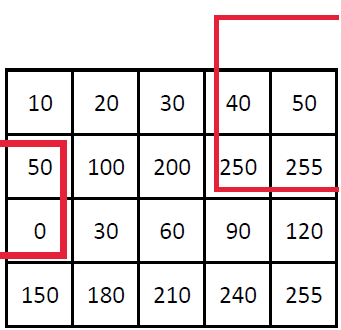
\includegraphics[width=.5\linewidth]{Image/Faltung/Faltung_original.png}
    \caption{Beispiel Graustufenbild}
    \label{fig:beispiel_matrix}     
    \end{minipage}
    \begin{minipage}[t]{.5\linewidth}
    \centering
    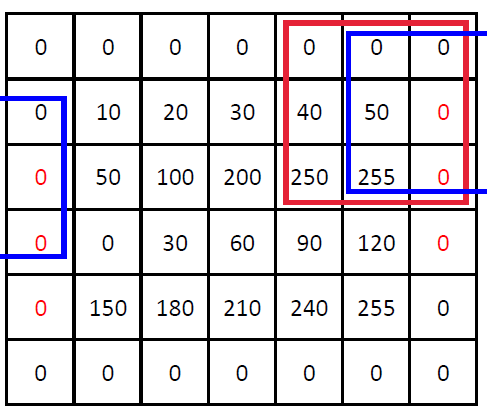
\includegraphics[width=.5\linewidth]{Image/Faltung/Faltung_padded.png}
    \caption{Graustufenbild nach Padding}
    \label{fig:matrix_nach_padding}
    \end{minipage}
\end{figure}
\newline
Um die zwei Probleme zu lösen, wird das Graustufenbild außenrum mit Nullen gepaddet und das gepaddete Bild hat eine Größe von $(x+2)\cdot(y+2)$ (siehe Abbildung \ref{fig:matrix_nach_padding}).\newline
1. So können alle Zugriffe außerhalb des Bildes vermieden werden (rotes Kästchen).\newline
2. Die Berechnung von Pixeln am Rand sind auch korrekt, allerdings diese Padding-Pixel und somit für uns irrelevant sind (blaues Kästchen).\newline
3. Während des Padding-Vorgangs können gleichzeitig die Pixel von 8 Bit zu 16 Bit integer konvertiert und gespeichert, um die Zwischenergebnisse korrekt darstellen zu können. Somit muss die Konvertierung nicht im Faltungsvorgang stattfinden.\newline
Wie in der Integer Implementierung werden Weichzeichnung und Kantendetektion in einem Durchgang berechnet. Anders als in \texttt{convolution} werden die Pixelwerte in \texttt{convolution\_simd} nicht in 8 Bit Integer zurückkonvertiert. Nach der Faltung müssen die Ergebnisse noch unpadded werden.

\item \textbf{Funktionsweise von \texttt{combine} in SIMD}\newline
Wie in \texttt{combine} nimmt \texttt{combine\_simd} die Ergebnisse von Weichzeichnung und Kantendetektion und setzte diese zusammen. Da die Zwischenergebnisse hier auch nicht in 8 Bit Integer dargestellt werden können, werden die Ergebnisse der Faltungen als 16 Bit Integer Array übergeben, was der Grund ist, warum auf die Rückkonvertierung auf 8 Bit Integer in \texttt{convolution\_simd} verzichtet wird. Neben der Rückkonvertierung findet hier auch der Unpadding-Vorgang statt, da die übergebene Ergebnisse der Faltung noch gepadded sind.
\end{itemize}
\section{Genauigkeit}
Durch die Speicherung in 8 Bit Integern ist das Ergebnis inhärent nur so präzise, wie es 8 Bit Integer darstellen können. Außerdem können sich – je nach Implementierung – Rundungsfehler ergeben. In diesem Kapitel werden diese Fehler und ihre Auswirkungen dargestellt. Eine Diskussion, ob diese Rundungsfehler angesichts der kürzeren Laufzeit akzeptabel sind, folgt in Kapitel 4.

\subsection{Korrektheitstests}
Mithilfe von Skripts in Matlab und Python wurden auf zufallszahlenbasierte Testdaten erstellt, um die einzelnen Unterfunktionen zu testen. Außerdem konnten die Ergebnisse der unterschiedlichen Implementation gleicher Funktionen verglichen werden, um Korrektheit sicherzustellen. Die oben genannten Rundungsungenauigkeiten führen hierbei nicht zum Fehlschlag, da die Tests bei den Implementierungen, die nicht auf Genauigkeit optimiert sind, Abweichungen der Pixelwerte im Ergebnis um +/-2 erlauben.

\subsection{Beispieleingaben}
Es wurden mit GIMP einige Bilder in das PPM-Format konvertiert, um sie anschließend zu entrauschen. Zur Erstellung der Bilder wurde teilweise der ISO-Wert der genutzten Kameras sehr hoch eingestellt, um starkes Bildrauschen hervorzurufen. Anhand dieser Bilder kann die Basisfunktionalität visuell überprüft und verglichen werden.
Da das Ergebnis in Graustufen ist, wurde hier zusätzlich das Eingabebild mit GIMP zu Graustufen konvertiert, um einen Vorher-Nachher-Vergleich zu vereinfachen.\newline
In den Abbildungen \ref{fig:eingabe}, \ref{fig:graustufen}, \ref{fig:entrauscht}, \ref{fig:detail_graustufen} und \ref{fig:detail_entrauscht}
sieht man den Effekt der Rauschreduzierung mit der vorausgewählten Implementierung. Es lassen sich einige Dinge direkt erkennen:
\begin{itemize}
\item \textbf{Graustufenkonvertierung:} das Programm hat das Bild sinnvoll zu Graustufen konvertiert, das Ergebnis ist vergleichbar mit der Konvertierung durch GIMP 

\item \textbf{Weichzeichnung:} Es lässt sich gut erkennen, dass das entrauschte Bild im Vergleich zum Eingabebild weichgezeichnet ist.

\item \textbf{Entrauschung:} Die Hauptfunktion des Programmes, Entrauschung, ist hier logischerweise auch erkennbar, besonders in der Detailansicht.
\end{itemize}
Neben den hier gezeigten Beispielen wurde das Programm mit verschiedenen Bilddateien getestet, um die korrekte Funktionsweise auch bei Randfällen sicherzustellen. Hierfür wurden neben alltagsnahen Beispielen auch Bilder verwendet, die ausgewählte Randfälle überprüfen. Es wurden beispielsweise sehr hochauflösende Bilder (ca. 100 Megapixel) oder solche mit unüblichen Seitenverhältnisse (2000:1) getestet. 
Bei keiner der Beispieleingaben wurden unerwartete Ergebnisse festgestellt.

\begin{figure}
    \centering
    \begin{minipage}[t]{.33\linewidth}
        \centering
        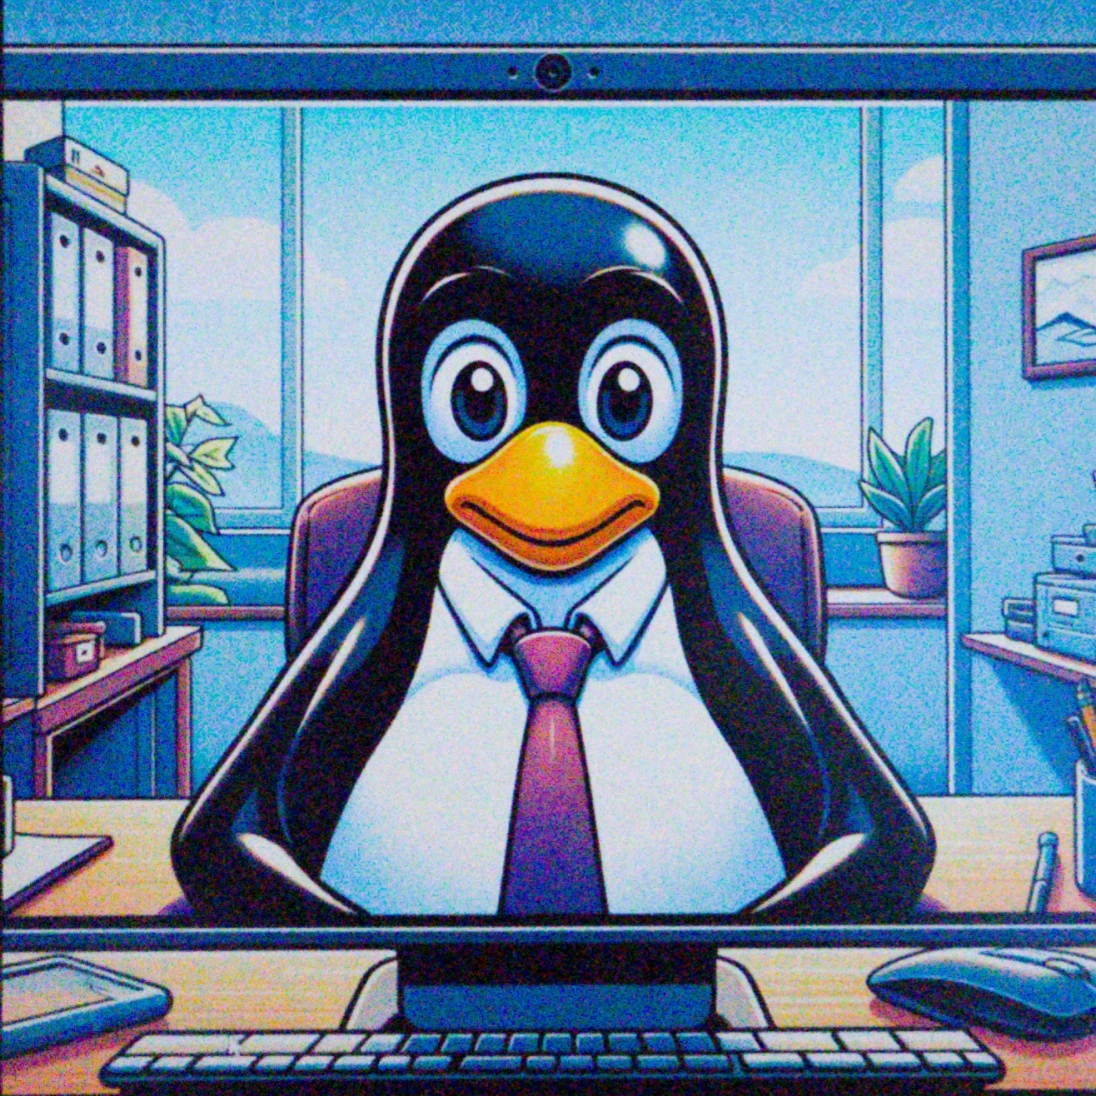
\includegraphics[width=\linewidth]{Image/Sample_VideoCall/noisyvideocall.png}
        \caption{Eingabe}
        \label{fig:eingabe}
    \end{minipage}%
    \begin{minipage}[t]{.33\linewidth}
        \centering
        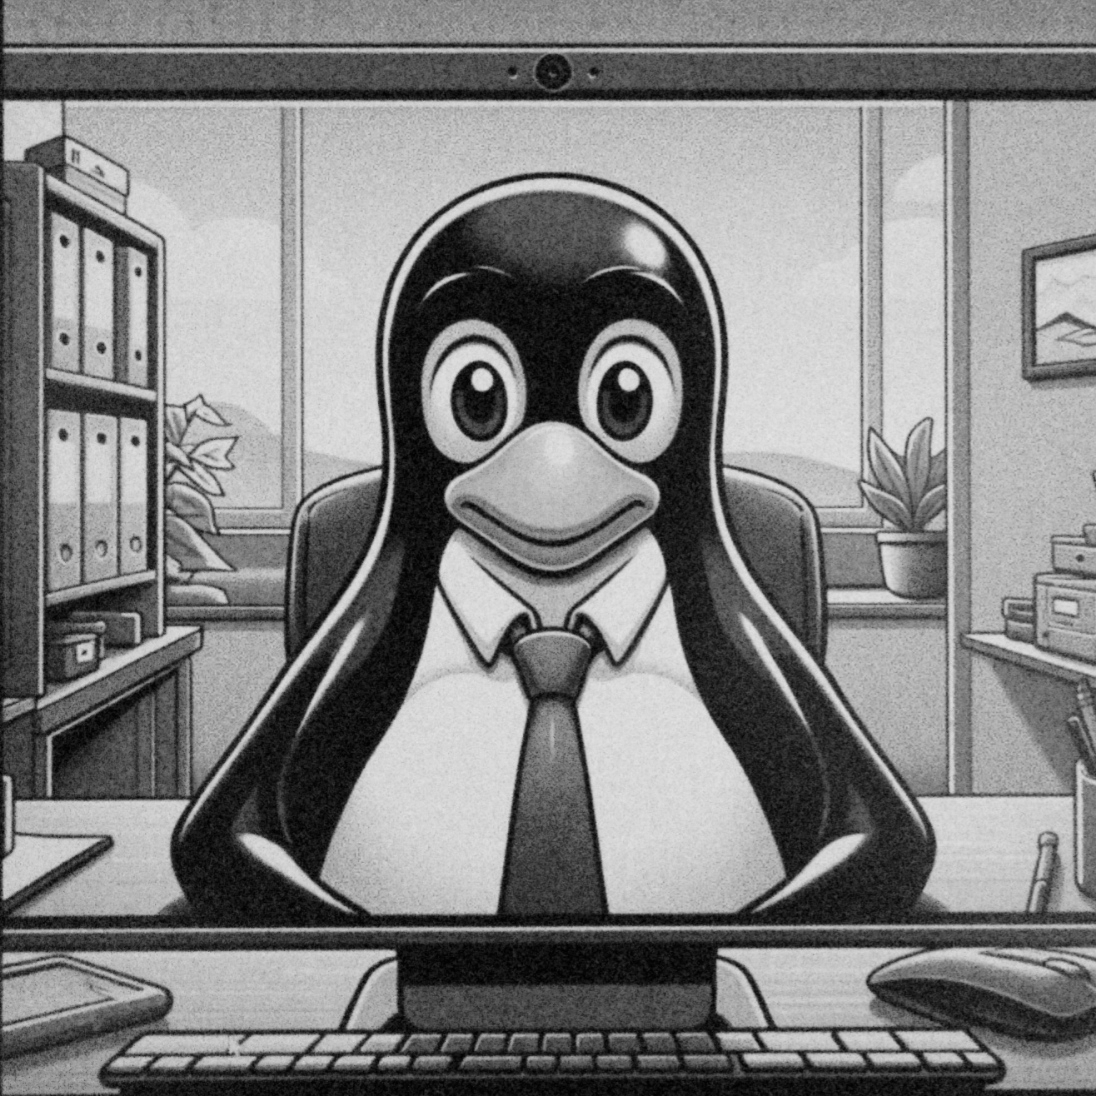
\includegraphics[width=\linewidth]{Image/Sample_VideoCall/noisyvideocall_greyscale.png}
        \caption{Graustufen}
        \label{fig:graustufen}
    \end{minipage}%
    \begin{minipage}[t]{.33\linewidth}
        \centering
        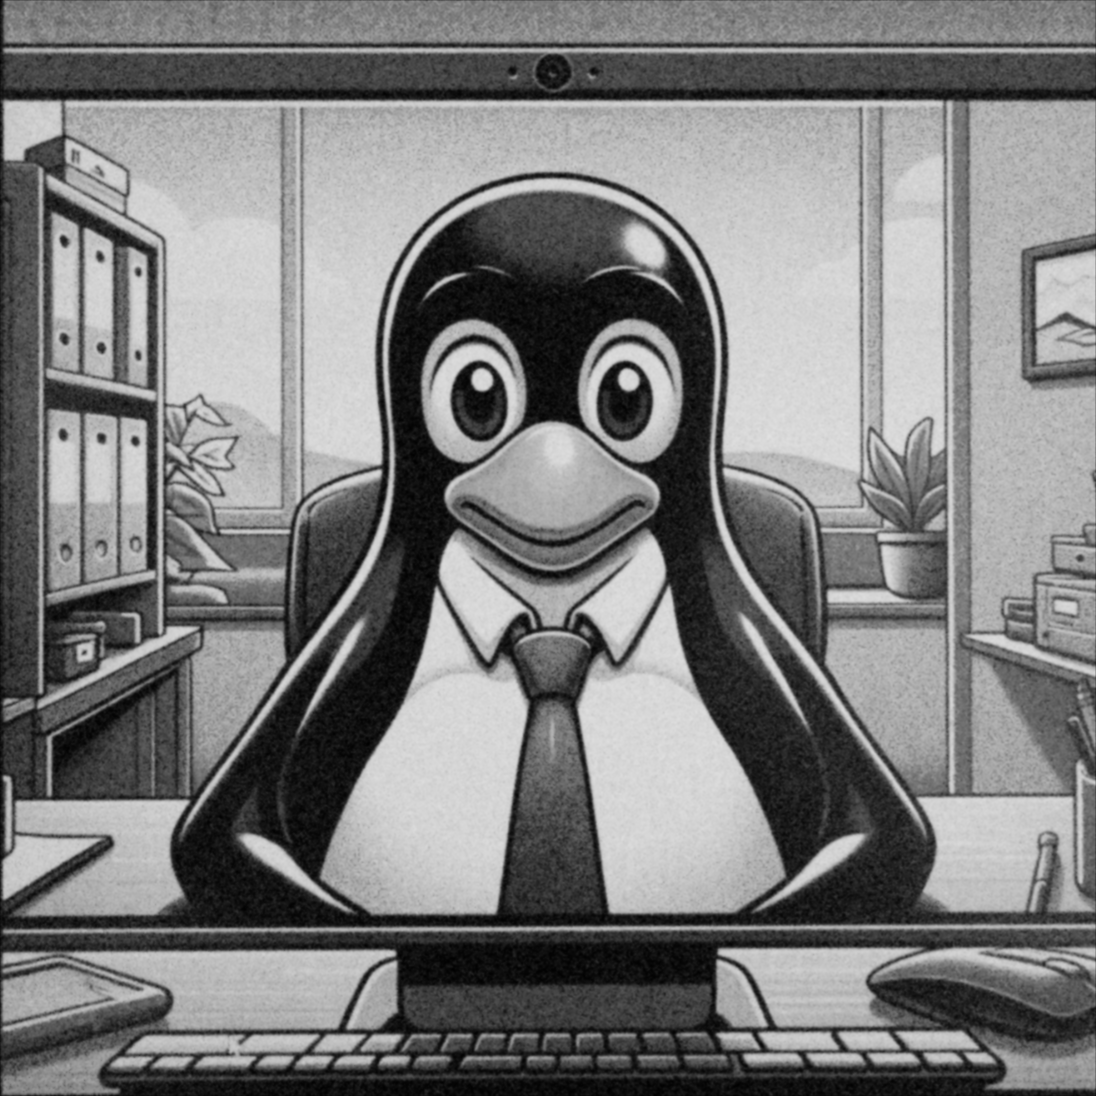
\includegraphics[width=\linewidth]{Image/Sample_VideoCall/denoisedvideocall_simd.png}
        \caption{Entrauscht}
        \label{fig:entrauscht}
    \end{minipage}
    \centering
    \begin{minipage}[t]{.33\linewidth}
        \centering
        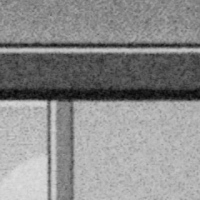
\includegraphics[width=\linewidth]{Image/Sample_VideoCall/noisyvideocall_detail.png}
        \caption{Graustufen}
        \label{fig:detail_graustufen}
    \end{minipage}%
    \begin{minipage}[t]{.33\linewidth}
        \centering
        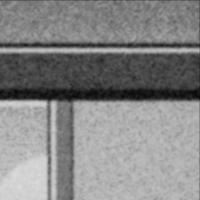
\includegraphics[width=\linewidth]{Image/Sample_VideoCall/denoisedvideocall_detail.png}
        \caption{Entrauscht}
        \label{fig:detail_entrauscht}
    \end{minipage}
\end{figure}



\subsection{Auswirkung der Genauigkeitsunterschiede}
In den Abbildungen \ref{fig:accurate}, \ref{fig:integer} und \ref{fig:simd}
können die Ergebnisse der verschiedenen Implementierungen an einer Beispieleingabe verglichen werden. Für das menschliche Auge sind kaum Unterschiede zwischen den Implementierungen erkennbar, auch wenn bei beiden beschleunigten Implementierungen mehr als 98 Prozent der Pixel einen anderen Wert als die genauere Implementierung haben.

\begin{figure}
    \centering
    \begin{minipage}[t]{.33\linewidth}
        \centering
        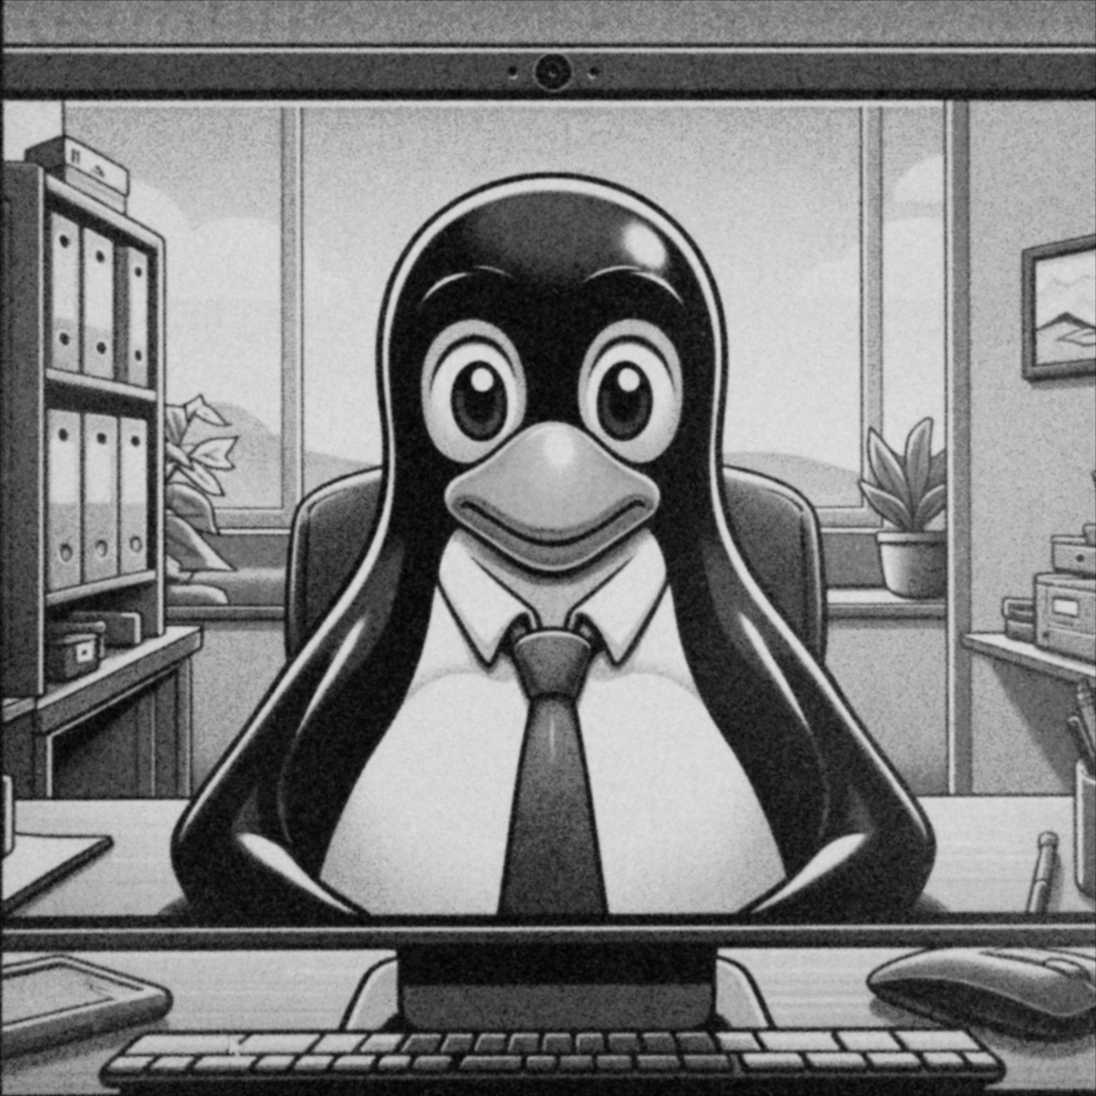
\includegraphics[width=\linewidth]{Image/Sample_VideoCall/denoisedvideocall_acurate.png}
        \caption{Accurate}
        \label{fig:accurate}
    \end{minipage}%
    \begin{minipage}[t]{.33\linewidth}
        \centering
        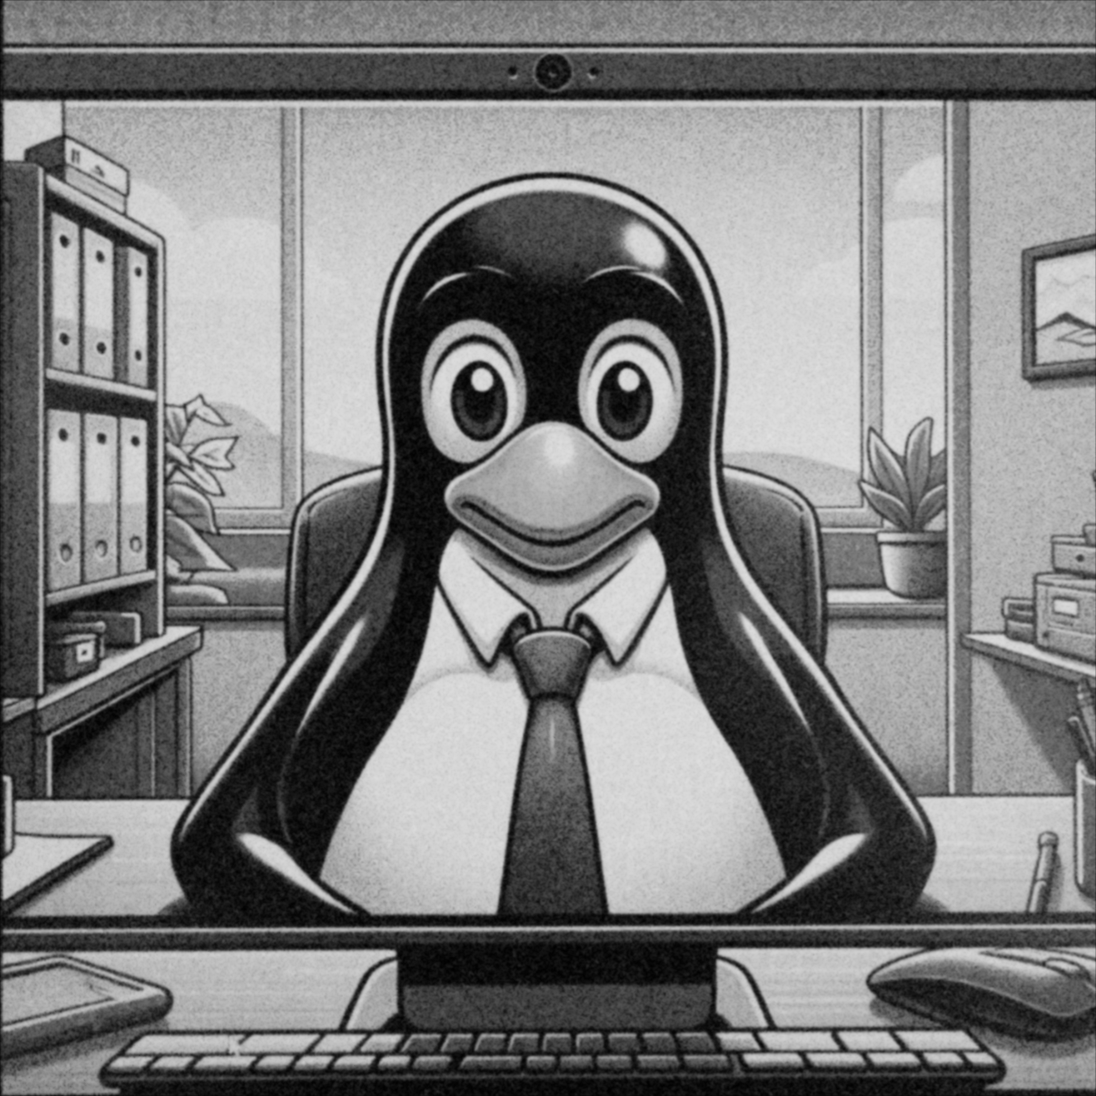
\includegraphics[width=\linewidth]{Image/Sample_VideoCall/denoisedvideocall_integer.png}
        \caption{Integer}
        \label{fig:integer}
    \end{minipage}%
    \begin{minipage}[t]{.33\linewidth}
        \centering
        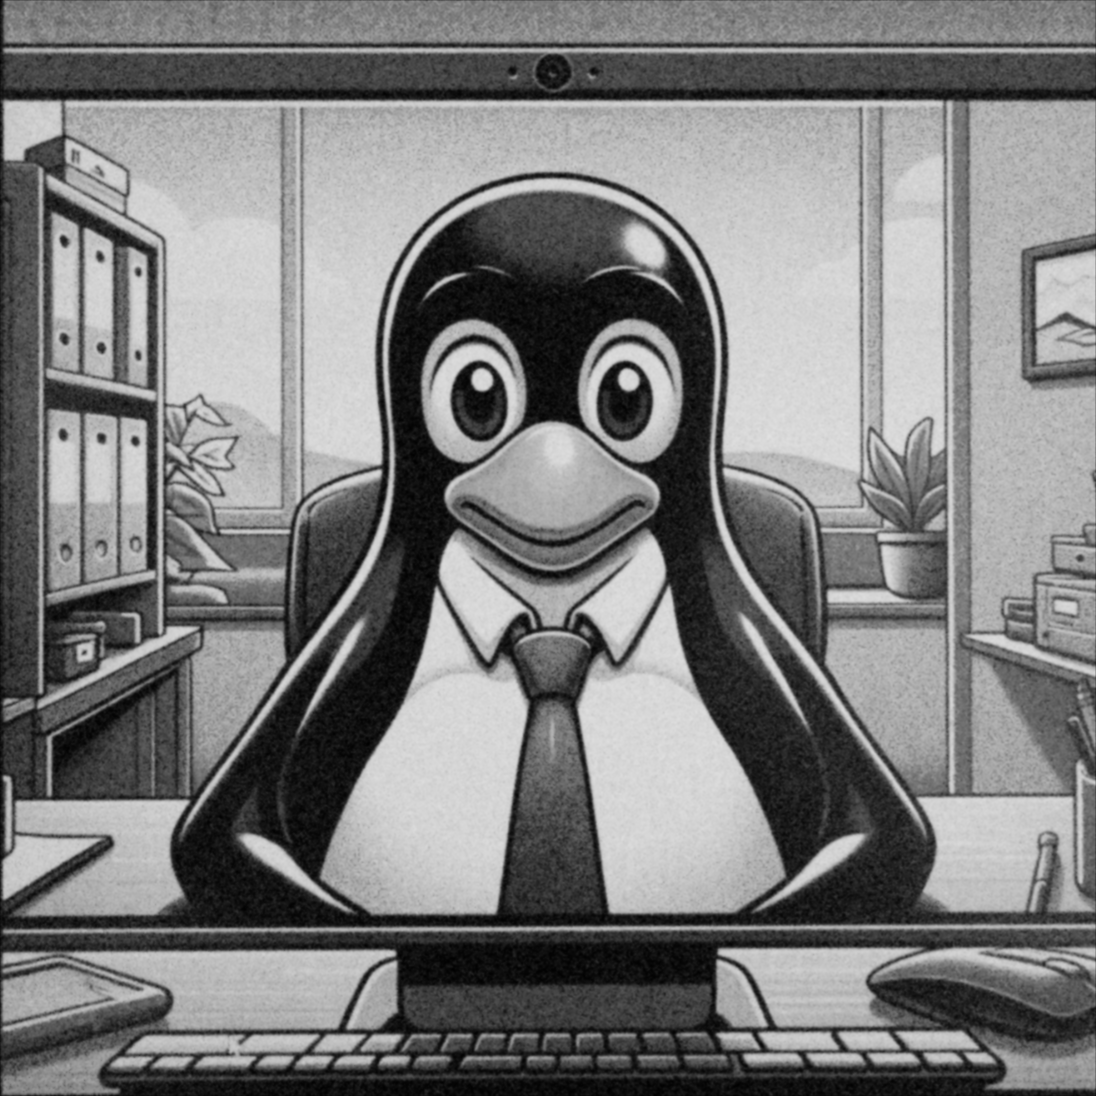
\includegraphics[width=\linewidth]{Image/Sample_VideoCall/denoisedvideocall_simd.png}
        \caption{SIMD}
        \label{fig:simd}
    \end{minipage}
\end{figure}

\section{Performanzanalyse}
%Messumgebung beschreiben

Für alle Zeitmessungen und das Profiling wurde das Programm auf einem Intel Core i7-8565U, 1,8 GHz, 16 GB RAM, Ubuntu LTS 22.04, Linux Kernel 6.5.0 ausgeführt. Kompiliert wurde mit GCC 11.4.0 mit der Option -O2.

\subsection{Vergleich der Optimierungsstufen bei verschiedenen Auflösungen}
Um die drei verschiedenen Implementierungen zu vergleichen, wurden Bilder mit zufälligen Pixeldaten mit einer Reihe unterschiedlicher Auflösungen generiert. Im Anschluss wurden für alle drei Implementierungen in Kombination mit jeder Auflösungsstufe die Laufzeit mit 50 Iterationen gemessen.
Die Verwendung von Integer Divisionen mit SISD beschleunigt die Berechnung durchschnittlich auf das 2,3-Fache, SIMD auf das 28,4-Fache. Die Abbildung \ref{fig:runtime} zeigen die Ergebnisse der Messung. Durch die logarithmische Skala auf der linken Seite lässt sich gut erkennen, dass die relative Laufzeit der Funktionen sich über die Auflösungen nur sehr leicht verändert. Bei allen drei Funktionen steigt die Laufzeit proportional zur Auflösung. Bei sehr kleinen Bildern ist die Integer-Implementierung vergleichsweise langsam, während die SIMD-Implementierung von kleineren Auflösungen im Vergleich zur akkuraten Implementierung von geringen Auflösungen profitiert. 

%TODO Nebeneinander
\begin{figure}
    \begin{minipage}[t]{.5\linewidth}
        \centering
        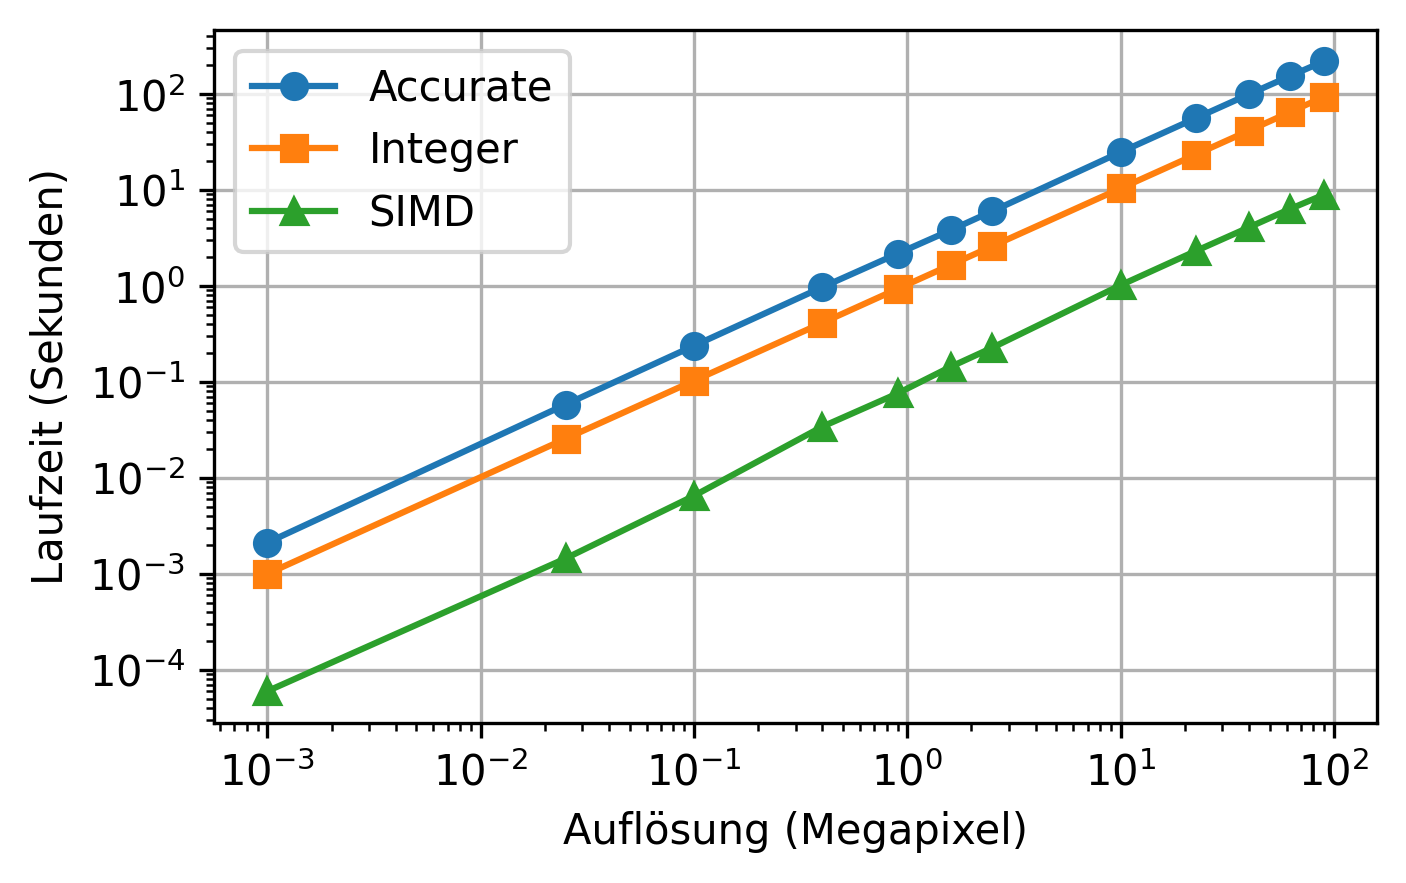
\includegraphics[width=\linewidth]{Image/Laufzeit/Laufzeit_log.png}
    \end{minipage}
    \begin{minipage}[t]{.5\linewidth}
        \centering
        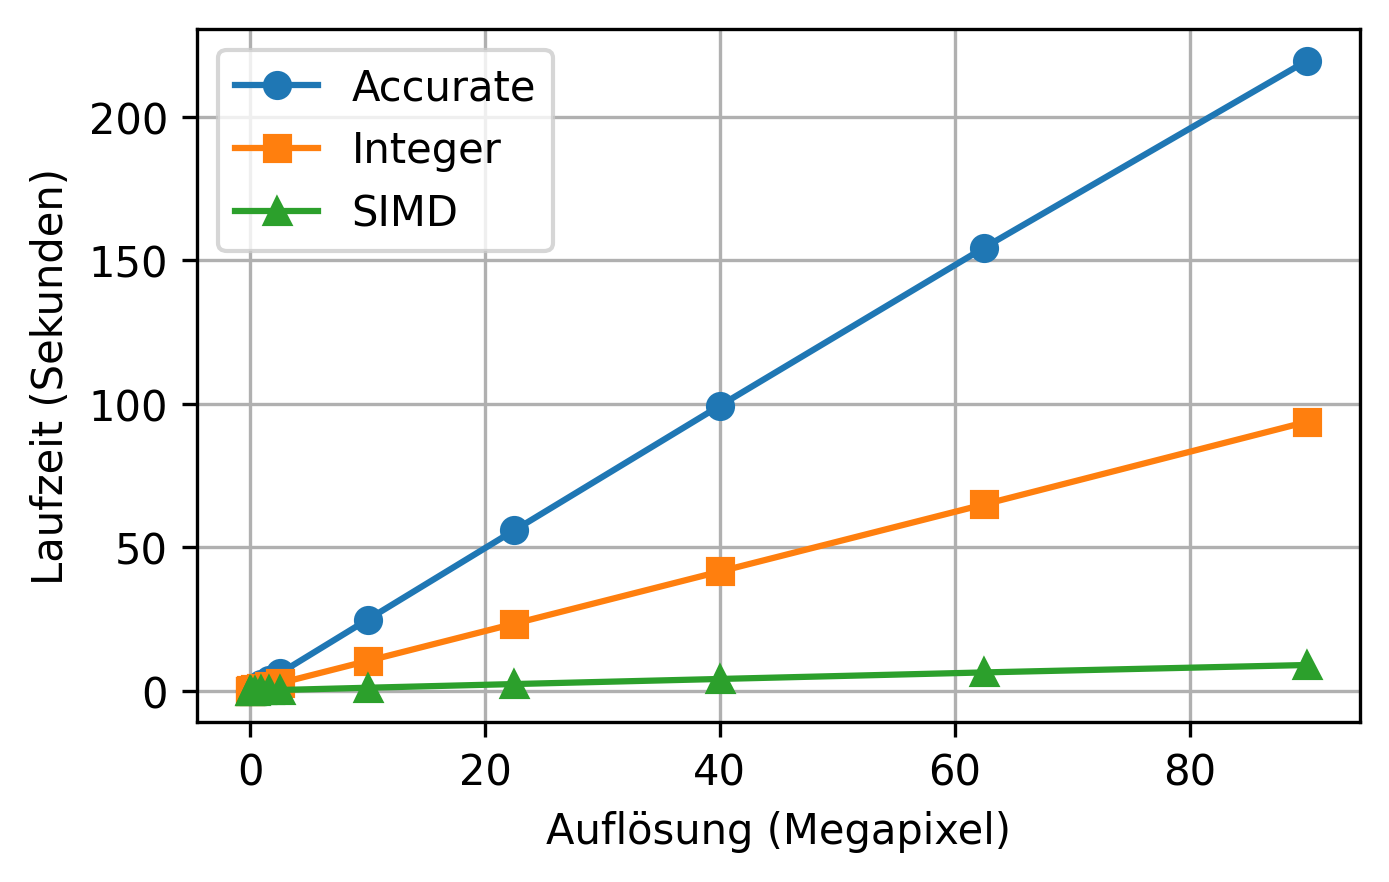
\includegraphics[width=\linewidth]{Image/Laufzeit/Laufzeit_linear.png}
    \end{minipage}
    \caption{Laufzeit bei verschiedenen Auflösungen (50 Iterationen, links logarithmische Skala, rechts Linear)}
    \label{fig:runtime}
\end{figure}

\subsection{Beispielhafter Performanzvergleich der Verwendung verschiedener Datentypen}
%Grayscale sisd vs Grayscale Integer um den Genauigkeit - Geschwindigkeit Tradeoff zu demonstrieren
Am Beispiel von der Funktion \texttt{grayscale} wurde getestet, welche Performance-Vorteile die Verwendung von Integer Division haben kann. Hierfür wurden eine kleine Auswahl Bilder mit jeweils 100 Iterationen zu Graustufen konvertiert. Die beiden Funktionen \texttt{grayscale} und \texttt{grayscale\_integer} sind bis auf die Unterschiede in der Verwendung von Ganzzahlarithmetik identisch.
Über alle getesteten Bilder war die Konvertierung mit Ganzzahlen im Durchschnitt um \textbf{49 Prozent} schneller als bei Verwendung von Fließkommazahlen. Diese Zahl zeigt exemplarisch, welche Vorteil die bewusste Verwendung der richtigen Datentypen haben kann. Es gilt abzuwägen, ob eine höhere Genauigkeit oder Performanz hier wichtiger ist.

\subsection{Wahl der Standardimplentierung}
Da die Genauigkeitsunterschiede wie in  den Abbildungen \ref{fig:accurate} und \ref{fig:integer} zu sehen bei der Bildentrauschung für das menschliche Auge kaum wahrnehmbar sind, wurde in Kombination mit den Ergebnissen aus Kapitel 4.1. entschieden, die SIMD-Version als Standardimplementierung zu verwenden. Die sehr großen Performanz-Vorteile überwiegen den Nachteil der leicht gesunkenen Genauigkeit.


\subsection{Profiling}
%Blick auf perf, welche Teilschritte den stärksten Optimierungsbedarf haben
Beim Profiling mittels \texttt{perf record} (Abbildung \ref{fig:profiling}) lässt sich erkennen, dass die Faltungen in der naiven Implementierung einen sehr hohen Anteil der Laufzeit ausmachen, während die Graustufenkonvertierung und finale Kombinierung im Vergleich sehr schnell sind. In der akkuraten Implementierung ist außerdem die Rundung ein relevanter Anteil, der in der Integer Version keine Rolle mehr spielt. Im Gegensatz zu den SISD-Imlementierungen ist in der SIMD-optimierten Lösung die Graustufenkonvertierung der größte Einzelfaktor. Da die RGB-Pixel als dreidimensionale Vektoren angeordnet sind, die zu einzelnen Werten zusammengefasst werden, können nur vier Pixel pro 128-Bit Register verarbeitet werden. Außerdem müssen hier zum Umordnen im Vergleich zu den anderen Funktionen mehr Instruktionen pro Pixel ausgeführt werden, um das Ergebnis zu erhalten. Deswegen lässt sich hier, anders als bei den anderen Funktionen, nur ein sehr viel kleinerer Performanzgewinn erreichen. 

\begin{figure}
    \centering
    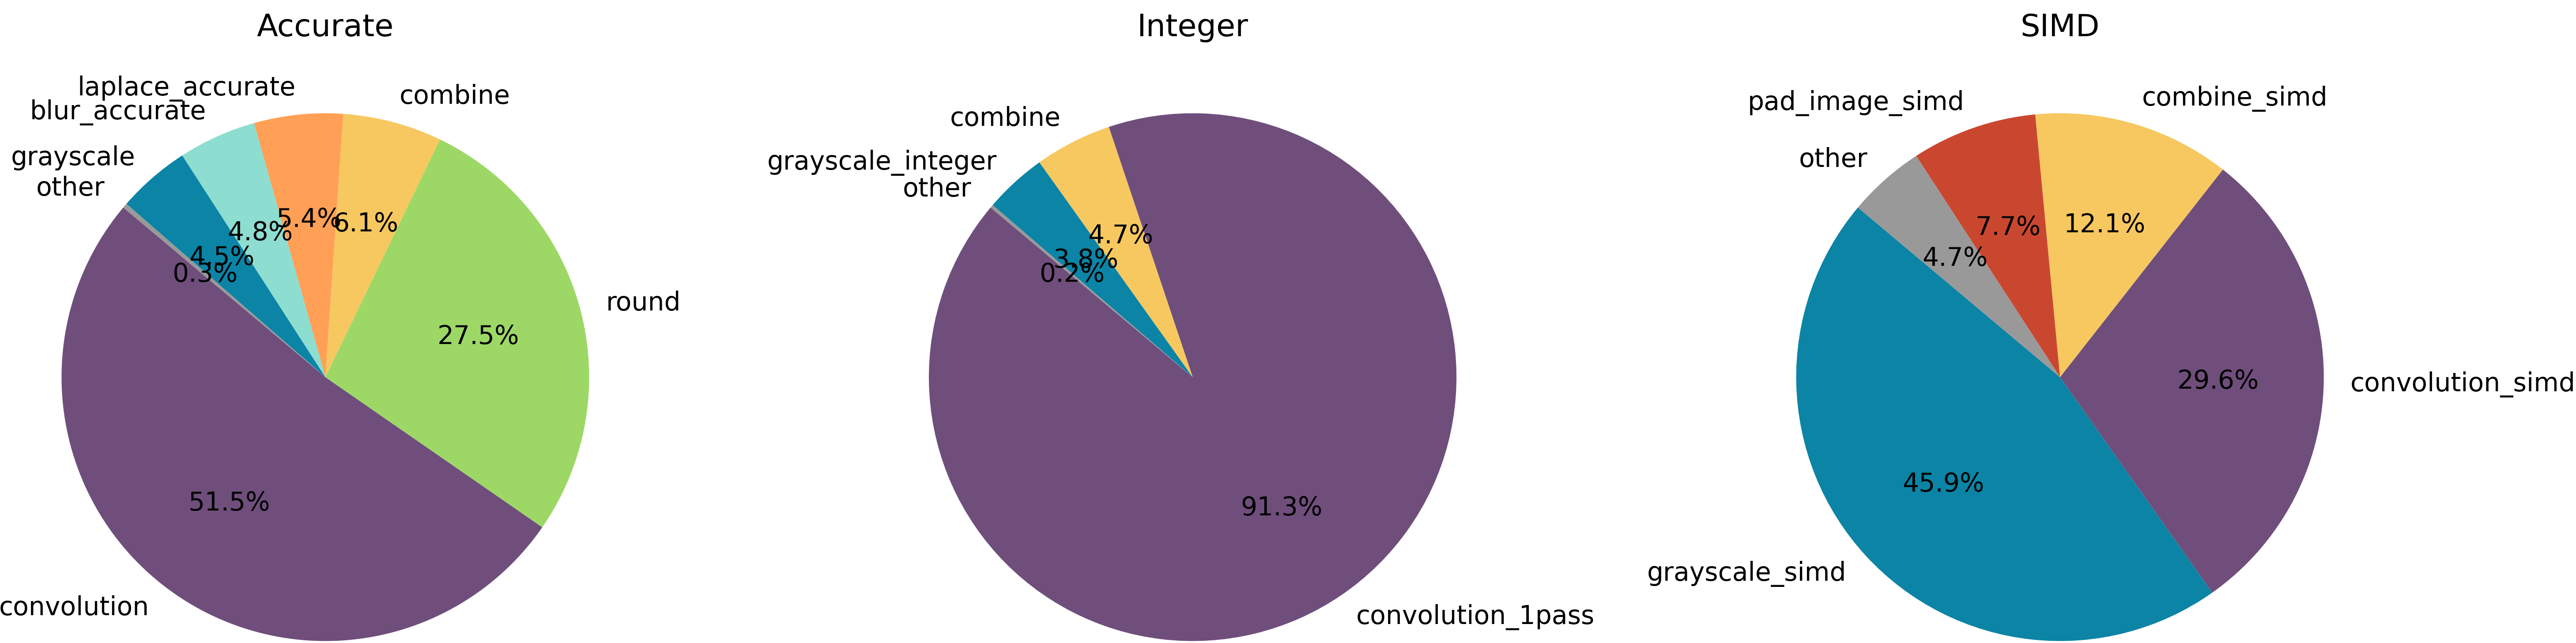
\includegraphics[width=\linewidth]{Image/Laufzeit/profiling.png}
    \caption{Prozentualer Anteil der einzelnen Funktionen an der Gesamtlaufzeit}
    \label{fig:profiling}
\end{figure}

%Diskussion, wie viel performance sinnvoll ist, Beispiel Videocall.
\subsection{Diskussion: Wie sinnvoll ist eine Optimierung?}
Der naive Ansatz benötigt selbst bei sehr hochauflösenden Bildern auf veralteten Laptop-Prozessoren weniger als eine Sekunde Rechenzeit. Die Optimierung einer Implementierung, wie sie hier durchgeführt wurde, ergibt vor allem dann Sinn, wenn sie im Kontext von Videos, speziell Echtzeit-Anwendungen wie Videoanrufen gesehen wird: Die optimierte Version könnte im Testsystem mehr als 200 Full-HD Bilder in der Sekunde entrauschen. Menschen empfinden Videos bereits bei 24 Bildern pro Sekunde als flüssig, eine zusätzliche Latenz von 5ms ist kaum wahrnehmbar. Ohne Optimierungen ließen sich ungefähr zehn Full-HD Bilder pro Sekunde entrauschen, das würde sich bei Echtzeitanwendungen nicht flüssig anfühlen. Hier hat die Optimierung mit SIMD also einen Anwendungsbereich erschlossen, der sonst nicht sinnvoll gewesen wäre.
\section{Zusammenfassung und Ausblick}
Die Implementierungsentscheidung wird maßgeblich durch die Balance zwischen Genauigkeit und Verarbeitungstempo determiniert: Eine präzise Implementierung sichert hohe Genauigkeit, beeinträchtigt jedoch das Verarbeitungstempo. Die Adaption einer Integer-Implementierung fördert die Prozessgeschwindigkeit unter Inkaufnahme von Genauigkeitsverlusten. SIMD-Instruktionen beschleunigen durch Parallelverarbeitung, können allerdings die intuitive Nachvollziehbarkeit einschränken.  Perspektivisch erscheint die Integration GPU-basierter Methoden zur Steigerung der Parallelverarbeitungskapazität vielversprechend.
% Zusammenfassende Aussage über drei Implemierungen
%Die präzise Implementierung gewährleistet hohe Genauigkeit, geht jedoch mit einer verlangsamten Verarbeitung einher. Die Nutzung einer Integer-Implementierung beschleunigt den Prozess, bringt jedoch gewisse Einbußen an Genauigkeit mit sich. Die SIMD-Version maximiert die Geschwindigkeit durch parallele Verarbeitung, wobei die intuitive Nachvollziehbarkeit der Prozesse leicht abnehmen kann. Insgesamt zeigt sich, dass die Wahl der Implementierung stark von den spezifischen Anforderungen an Genauigkeit und Geschwindigkeit abhängt. Beachtenswert ist, dass SIMD besonders gut für die Bildverarbeitung geeignet ist. In der vorliegenden Umsetzung wurde ausschließlich SSE verwendet, welches lediglich 128-Bit-Register zur Verfügung stellt. Ein vielversprechender Ausblick besteht in der Erwägung der Integration von GPU-basierten Ansätzen, um die Parallelität weiter zu optimieren.
%Der gewählte Entrauschungsalgorithmus zeichnet sich durch seine Einfachheit und Effektivität aus. Die Implementierung gestaltet sich unkompliziert, was auf die klare Struktur des Algorithmus zurückzuführen ist. Da der Algorithmus auf Weichzeichnung basiert, ist es unvermeidlich, dass das entrauschte Bild eine geringere Auflösung aufweist als das Original. In der aktuellen Zeit gewinnt das Entrauschen mithilfe von KI an Poularität, erfordert jedoch eine leistungsfähige GPU.
% Bildverarbeiting mit SIMD super gut parallelizierbar. Ausblick GPU
% Vor- und Nachteile des Algorithmus: 
% Einfach zu implementiren, Simple aber effective Algorithmus 
% Trade off Auflösung Einfachheit/Geschwindigket, Ausblick entrauschen mit KI


\newpage
\bibliographystyle{plain}
\bibliography{Ausarbeitung}{}

\end{document}
